\documentclass[12pt]{article}

\usepackage{amsmath, amssymb}
\usepackage[margin=1in]{geometry}
\usepackage{helvet}
\renewcommand{\familydefault}{\sfdefault}
\def\newrule#1#2#3{\begin{center}
    {#1} \\
    \line(1,0){300} {}{}{}{}{}{}{} [{#3}]\\
    {#2}
\end{center}}

\begin{document}
\def\assignment{AI Proposal}

\pagenumbering{gobble}
\noindent{\large COSC 4955 \hfill Name: \underline{Andey Tuttle} \\ Senior Design}
\begin{center}
    {\Large \assignment} \\ \textbf{\today}
\end{center}


\vspace{2em}

This document details a proposal for the combinational and learning AI that will play a major role in the game Sasq-watch, developed by Cryptid Games.

\section{High Level Overview}

The AI will be made up of three components, detailed below. Each of these components is a stripped down model of certain AI principles, namely a neural network, a genetic combination algorithm, and a recurrent neural network.

\begin{enumerate}
    \item A state machine with transfer weights in the graph determined by a vector given to the state machine at the start of the game
    \item A combination algorithm which takes the personal weight vectors of each player and joins them into one weight vector for propogation into the state machine. This combinational algorithm will also be used to combine each player's weight vector with the modified game vector created after the learning phase.
    \item A "learning phase" algorithm that, after being successfully defeated, goes back through the weight vector and modifies weights to direct the AI in a different direction, preventing the same attack from being successfully executed in the same way again.
\end{enumerate}

The aim with these components is to simulate, at the high level, the same processes that make recurrent nerual networks highly efficient at learning when presented with vast sums of training data and plenty of computation time are being stripped down and manually guided so that they can be applied to a hand-crafted game experience.

\section{State Machine}

The state machine sits in a place halfway between a state machine and a neural network. Figure \ref{fig:state1} is an example of a very small machine that will be used for discussion purposes. 

\begin{figure}
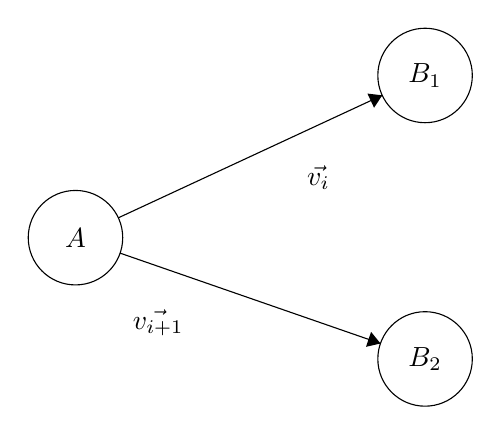
\begin{tikzpicture}[scale=0.2]
\tikzstyle{every node}+=[inner sep=0pt]
\draw [black] (12.6,-16.8) circle (3);
\draw (12.6,-16.8) node {$A$};
\draw [black] (34.8,-6.5) circle (3);
\draw (34.8,-6.5) node {$B_1$};
\draw [black] (34.8,-24.5) circle (3);
\draw (34.8,-24.5) node {$B_2$};
\draw [black] (15.32,-15.54) -- (32.08,-7.76);
\fill [black] (32.08,-7.76) -- (31.14,-7.65) -- (31.56,-8.55);
\draw (28.03,-12.18) node [below] {$\vec{v_i}$};
\draw [black] (15.43,-17.78) -- (31.97,-23.52);
\fill [black] (31.97,-23.52) -- (31.37,-22.78) -- (31.05,-23.73);
\draw (17.86,-21.36) node [below] {$\vec{v_{i+1}}$};
\end{tikzpicture}
\caption{An example state machine for discussion}
\label{fig:state1}
\end{figure}

State $A$ represents a specific behavior of the cryptid, while states $B_1$ and $B_2$ are two behaviors that can occur from state $A$. $\vec{v_i}$ refers to the $i$th value in $\vec{v}$. State A is made up of two components: a cryptid action function and a transfer decision function. The cryptid action function describes the behavior that the cryptid will perform (i.e. forrage, travel, sleep, etc.). This is the main function of how the state machine interacts with the game, which allows us to leverage pre-existing knowledge and resources for Unity to simply create the AI using a state machine. The second component, the transfer decision function could work in one of two ways.

The first way it could work is very similar to the way a neural network moves through its weights. The decision function outputs a number $n$ such that $n \in [-1, 1]$. $\vec{v_i}$ could remain normal while $\vec{v_{i+1}}$ is negated. Then, the state transfers anytime the transfer function evaluates to a value above $\vec{v_i}$ or below $\vec{v_{i+1}}$. This design could also work by assigning ranges to each edge of the state machine's graph with a specific range dedicated for the "remain in this state" decision. I believe this would be the worse of the two options because it limits the number of possible states we can transfer to, and it requires incredibly complex transfer functions.

The second way it could work is by having the transfer function provide a binary conclusion of transfer or stay. Then, when it decides on a transfer, the weights of all outgoing edges serve as the ratios for transfers. For example, the transfer from state $A$ would transfer to state $B_1$ with probability $P(\vec{v_i})$ and would transfer to state $B_2$ with probability $P(\vec{v_{i+1}})$. This allows for non-deterministic actions from the cryptid, and the computation of state transfers will be far less significant.

\section{Vector Combination Algorithm}

The vector combination algorithm fulfills several roles in the game. First, it allows four players joining the game to combine their individual cryptid decision vectors in a non-deterministic way, and it allows for the group decision vector to be combined with individual player vector after the game, letting the game affect future games. The combination algorithm is going to be similar to the genetic combination algorithms present in genetic learning alrogithms. The table below demonstrates this phenomenon.

\begin{tabular}{ccccc}
$\vec{v_0}$ & & $\vec{u_0}$ & & $\vec{v_0}$ \\
$\vec{v_1}$ & & $\vec{u_1}$ & $\Longrightarrow$ & $\vec{u_1}$ \\
$\vec{v_2}$ & & $\vec{u_2}$ & & $\vec{u_2}$ \\
\vdots & & & & \\
$\vec{v_n}$ & & $\vec{u_n}$ & & $\vec{v_n}$ \\
\end{tabular}

The first element in each vector will be a simple count of the number of games a vector has "played" in. In this way, the combination algorithm can weight the cross pollination of "genes" based upon how "experienced" that vector is. The combination of the first two values could, for example, take the form of the equation:

\begin{equation}
    \frac{{\log_{10}(\vec{v_0})}\vec{v_1} + {\log_{10}(\vec{u_0})}\vec{u_1}}{\log_{10}(\vec{v_0}) + \log_{10}(\vec{u_0})} = \vec{game_1}
\end{equation}

Then, after the games conclusion, to update a player's weight vector, the same calculation can be performed with $\vec{game}$ taking the place of $\vec{v}$ in the equation above and the weight ratios being the ratio between total games played by all players and total games played by this player. 

\section{Learning Algorithm}

The learning algorithm takes advantage of the fact that a state machine is really just a graph. As the game runs, every state transition pushes the state onto a stack. Then, when the game is finished, we can assume that the last few transitions led to the game loss. Therefore, we step back through the states and adjust the weights that allow arriving in those states. Then, we can perform a simple graph traversal to see if it becomes more difficult to arrive at that state through a given transition. If it does, then we consider it a successful change and continue to "prune" the next element on the stack by performing the same action. This can be repeated for a variable depth, allowing us to modify the amount of the game that is modified each time. A possible solution is that the depth is inversely related to how many games have been played.

\end{document}